% Options for packages loaded elsewhere
\PassOptionsToPackage{unicode}{hyperref}
\PassOptionsToPackage{hyphens}{url}
%
\documentclass[
  ignorenonframetext,
  aspectratio=43,
]{beamer}
\usepackage{pgfpages}
\setbeamertemplate{caption}[numbered]
\setbeamertemplate{caption label separator}{: }
\setbeamercolor{caption name}{fg=normal text.fg}
\beamertemplatenavigationsymbolsempty
% Prevent slide breaks in the middle of a paragraph
\widowpenalties 1 10000
\raggedbottom
\setbeamertemplate{part page}{
  \centering
  \begin{beamercolorbox}[sep=16pt,center]{part title}
    \usebeamerfont{part title}\insertpart\par
  \end{beamercolorbox}
}
\setbeamertemplate{section page}{
  \centering
  \begin{beamercolorbox}[sep=12pt,center]{part title}
    \usebeamerfont{section title}\insertsection\par
  \end{beamercolorbox}
}
\setbeamertemplate{subsection page}{
  \centering
  \begin{beamercolorbox}[sep=8pt,center]{part title}
    \usebeamerfont{subsection title}\insertsubsection\par
  \end{beamercolorbox}
}
\AtBeginPart{
  \frame{\partpage}
}
\AtBeginSection{
  \ifbibliography
  \else
    \frame{\sectionpage}
  \fi
}
\AtBeginSubsection{
  \frame{\subsectionpage}
}

\usepackage{amsmath,amssymb}
\usepackage{iftex}
\ifPDFTeX
  \usepackage[T1]{fontenc}
  \usepackage[utf8]{inputenc}
  \usepackage{textcomp} % provide euro and other symbols
\else % if luatex or xetex
  \usepackage{unicode-math}
  \defaultfontfeatures{Scale=MatchLowercase}
  \defaultfontfeatures[\rmfamily]{Ligatures=TeX,Scale=1}
\fi
\usepackage{lmodern}
\ifPDFTeX\else  
    % xetex/luatex font selection
\fi
% Use upquote if available, for straight quotes in verbatim environments
\IfFileExists{upquote.sty}{\usepackage{upquote}}{}
\IfFileExists{microtype.sty}{% use microtype if available
  \usepackage[]{microtype}
  \UseMicrotypeSet[protrusion]{basicmath} % disable protrusion for tt fonts
}{}
\makeatletter
\@ifundefined{KOMAClassName}{% if non-KOMA class
  \IfFileExists{parskip.sty}{%
    \usepackage{parskip}
  }{% else
    \setlength{\parindent}{0pt}
    \setlength{\parskip}{6pt plus 2pt minus 1pt}}
}{% if KOMA class
  \KOMAoptions{parskip=half}}
\makeatother
\usepackage{xcolor}
\newif\ifbibliography
\setlength{\emergencystretch}{3em} % prevent overfull lines
\setcounter{secnumdepth}{-\maxdimen} % remove section numbering


\providecommand{\tightlist}{%
  \setlength{\itemsep}{0pt}\setlength{\parskip}{0pt}}\usepackage{longtable,booktabs,array}
\usepackage{calc} % for calculating minipage widths
\usepackage{caption}
% Make caption package work with longtable
\makeatletter
\def\fnum@table{\tablename~\thetable}
\makeatother
\usepackage{graphicx}
\makeatletter
\def\maxwidth{\ifdim\Gin@nat@width>\linewidth\linewidth\else\Gin@nat@width\fi}
\def\maxheight{\ifdim\Gin@nat@height>\textheight\textheight\else\Gin@nat@height\fi}
\makeatother
% Scale images if necessary, so that they will not overflow the page
% margins by default, and it is still possible to overwrite the defaults
% using explicit options in \includegraphics[width, height, ...]{}
\setkeys{Gin}{width=\maxwidth,height=\maxheight,keepaspectratio}
% Set default figure placement to htbp
\makeatletter
\def\fps@figure{htbp}
\makeatother

\makeatletter
\@ifpackageloaded{caption}{}{\usepackage{caption}}
\AtBeginDocument{%
\ifdefined\contentsname
  \renewcommand*\contentsname{Table of contents}
\else
  \newcommand\contentsname{Table of contents}
\fi
\ifdefined\listfigurename
  \renewcommand*\listfigurename{List of Figures}
\else
  \newcommand\listfigurename{List of Figures}
\fi
\ifdefined\listtablename
  \renewcommand*\listtablename{List of Tables}
\else
  \newcommand\listtablename{List of Tables}
\fi
\ifdefined\figurename
  \renewcommand*\figurename{Figure}
\else
  \newcommand\figurename{Figure}
\fi
\ifdefined\tablename
  \renewcommand*\tablename{Table}
\else
  \newcommand\tablename{Table}
\fi
}
\@ifpackageloaded{float}{}{\usepackage{float}}
\floatstyle{ruled}
\@ifundefined{c@chapter}{\newfloat{codelisting}{h}{lop}}{\newfloat{codelisting}{h}{lop}[chapter]}
\floatname{codelisting}{Listing}
\newcommand*\listoflistings{\listof{codelisting}{List of Listings}}
\makeatother
\makeatletter
\makeatother
\makeatletter
\@ifpackageloaded{caption}{}{\usepackage{caption}}
\@ifpackageloaded{subcaption}{}{\usepackage{subcaption}}
\makeatother

\ifLuaTeX
  \usepackage{selnolig}  % disable illegal ligatures
\fi
\usepackage{bookmark}

\IfFileExists{xurl.sty}{\usepackage{xurl}}{} % add URL line breaks if available
\urlstyle{same} % disable monospaced font for URLs
\hypersetup{
  pdftitle={Log Transformations},
  pdfauthor={Foundations of Regression and Predictive Modeling},
  hidelinks,
  pdfcreator={LaTeX via pandoc}}


\title{Log Transformations}
\subtitle{Growth rates, percent errors, and elasticity}
\author{Foundations of Regression and Predictive Modeling}
\date{}
\institute{James Scott \textbar{} Abhra Sarkar \textbar{} UT-Austin}

\begin{document}
\frame{\titlepage}


\begin{frame}{A straight line is a promise}
\phantomsection\label{a-straight-line-is-a-promise}
In simple linear regression, a slope means:

\begin{quote}
Add this much to \(y\) for one more unit of \(x\).
\end{quote}

Examples:

\begin{itemize}
\tightlist
\item
  one more year of age: subtract about 0.7 BPM,
\item
  one more square foot: add \$500 to house price.
\end{itemize}

One-unit change in \(x\), \(\beta_1\)-unit change in \(y\), no matter
the value of \(x\).
\end{frame}

\begin{frame}{March 2014}
\phantomsection\label{march-2014}
On March 23, 2014, WHO announced an outbreak of Ebola virus disease in
Guinea.

Imagine we are sitting in an outbreak-response meeting.

\begin{quote}
If this keeps going, how many cases are we looking at next month?
\end{quote}

We need a model before the situation outruns our intuition.
\end{frame}

\begin{frame}{A bad first instinct}
\phantomsection\label{a-bad-first-instinct}
Here's what lab-confirmed case looked like from March 23.

\begin{figure}[H]

{\centering 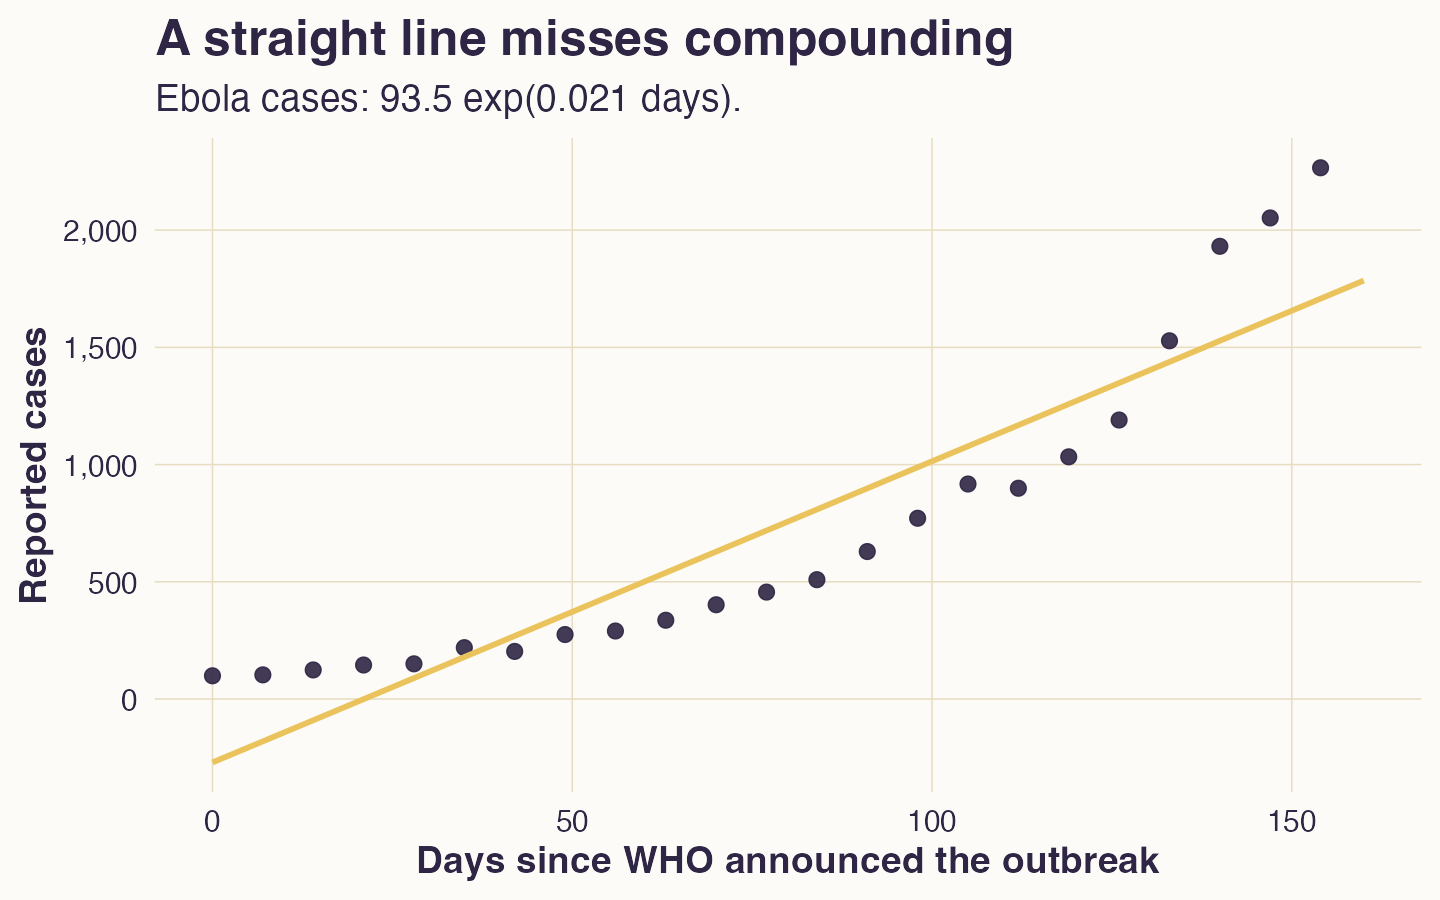
\includegraphics[width=0.86\textwidth,height=\textheight]{assets/epidemic-linear-bad.png}

}

\caption{Scatterplot of Ebola cases over time since WHO announced the
outbreak, with a straight-line fit that misses the compounding growth.}

\end{figure}%
\end{frame}

\begin{frame}{What the straight line says}
\phantomsection\label{what-the-straight-line-says}
A straight line forces one answer:

\begin{quote}
Each additional day adds the same number of cases.
\end{quote}

That means:

\begin{itemize}
\tightlist
\item
  day 10 to day 11: add \(c\) cases,
\item
  day 80 to day 81: add \(c\) cases,
\item
  And so on.
\end{itemize}

But the outbreak is not adding the same number each day. It is
compounding.
\end{frame}

\begin{frame}{The model we want}
\phantomsection\label{the-model-we-want}
For early epidemic growth, the natural model is:

\begin{quote}
Each day, the case count is multiplied by roughly the same factor.
\end{quote}

In this data set, it turns out that:

\[
\frac{\text{cases tomorrow}}{\text{cases today}} \approx 1.021.
\]

That is 2.1\% growth per day. \textbf{How did we determine that?}
\end{frame}

\begin{frame}{The exponential model}
\phantomsection\label{the-exponential-model}
The exponential model expresses this as:

\[
Y_t = Y_0 e^{rt}.
\]

\begin{itemize}
\tightlist
\item
  \(Y_0\): initial count at time \(t=0\).
\item
  \(Y_t\): expected count after \(t\) days.
\item
  \(r\): daily growth rate.
\item
  \(t\): days since the outbreak announcement.
\end{itemize}

For this example:

\[
Y_t = 93.5e^{0.021t}.
\]
\end{frame}

\begin{frame}{The curve fits the story}
\phantomsection\label{the-curve-fits-the-story}
\begin{figure}[H]

{\centering 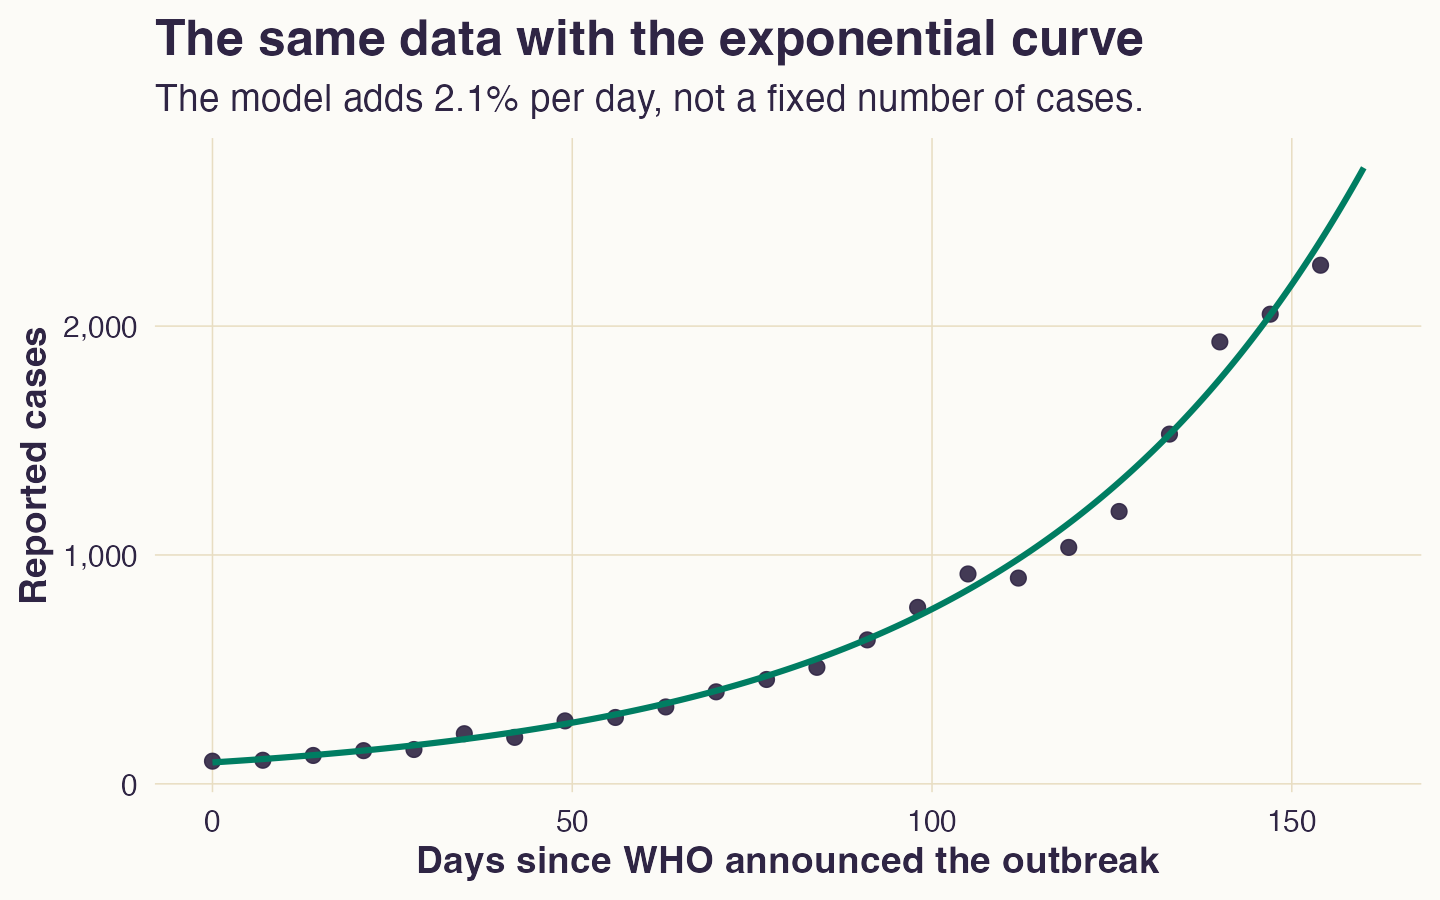
\includegraphics[width=0.86\textwidth,height=\textheight]{assets/epidemic-exponential-fit.png}

}

\caption{Scatterplot of Ebola cases by days since WHO announced the
outbreak, with the fitted exponential curve.}

\end{figure}%
\end{frame}

\begin{frame}{So are we stuck?}
\phantomsection\label{so-are-we-stuck}
No.~Logs turn multiplication into addition:

\[
\log(a \cdot b) = \log(a) + \log(b).
\]

Start with the exponential model:

\[
Y_t = Y_0e^{rt}.
\]

Take logs:

\[
\log(Y_t) = \log(Y_0) + rt.
\]

Now we have a straight-line model.
\end{frame}

\begin{frame}{The same data on the log scale}
\phantomsection\label{the-same-data-on-the-log-scale}
\begin{figure}[H]

{\centering 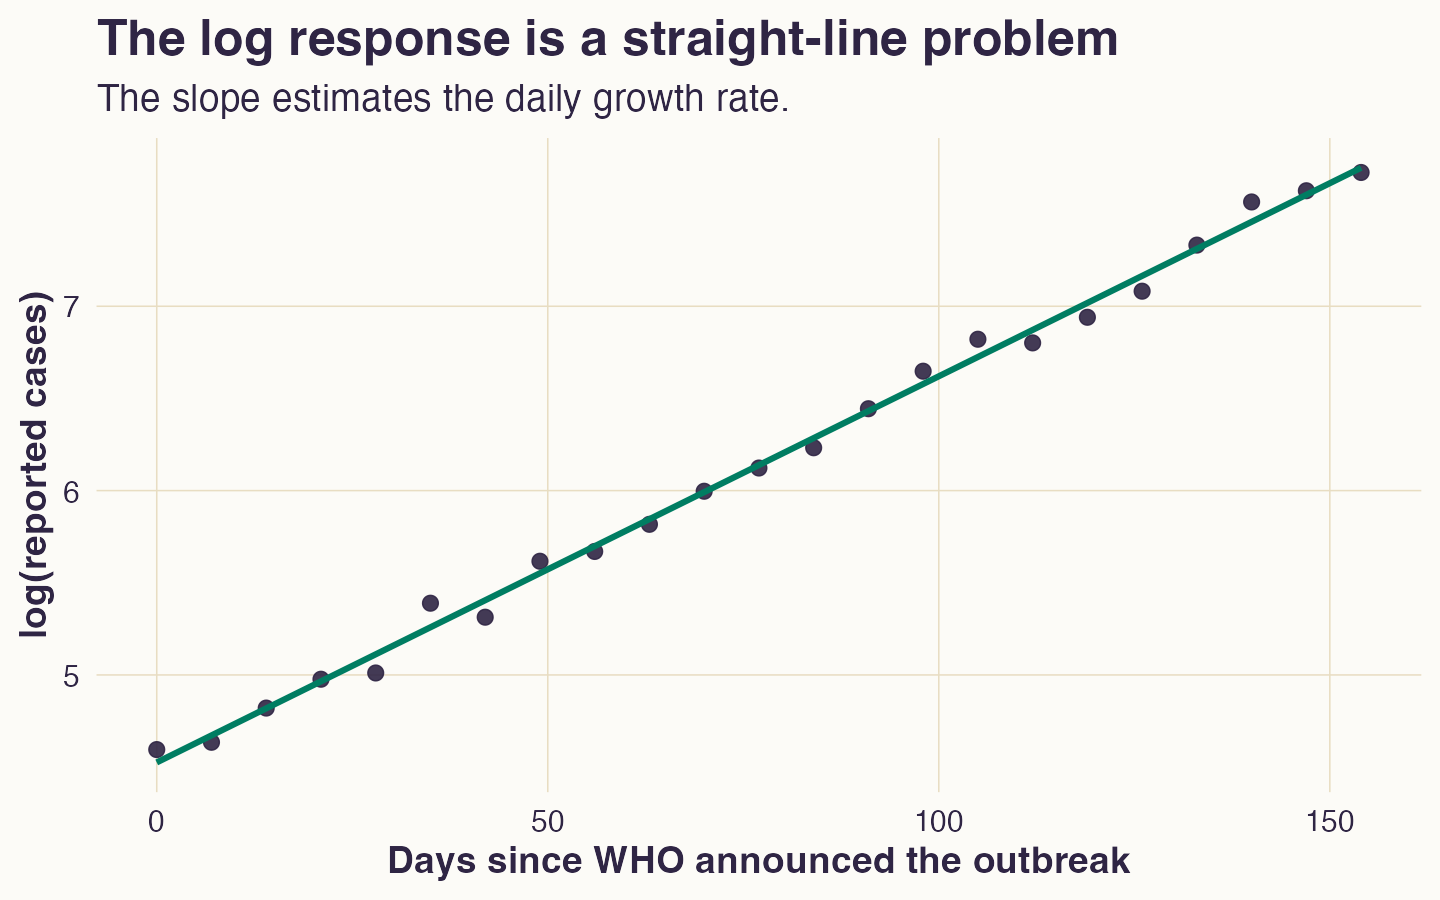
\includegraphics[width=0.86\textwidth,height=\textheight]{assets/epidemic-log-fit.png}

}

\caption{Scatterplot of log Ebola cases versus days since WHO announced
the outbreak, with a fitted line.}

\end{figure}%
\end{frame}

\begin{frame}{What the fitted line means}
\phantomsection\label{what-the-fitted-line-means}
On the log scale, the fitted equation is approximately:

\[
\widehat{\log(\text{cases})} = 4.53 + 0.021 \cdot \text{day}.
\]

Translation:

\begin{itemize}
\tightlist
\item
  \(4.54\) is the starting log count,
\item
  \(0.021\) is the daily log-growth rate,
\item
  \(e^{0.021} \approx 1.021\): the fitted count multiplies by about
  1.021 each day.
\end{itemize}

The slope is the percentage change each time period.
\end{frame}

\begin{frame}{Comparing scales}
\phantomsection\label{comparing-scales}
On the log scale:

\[
\widehat{\log(\text{cases})} = 4.53 + 0.021 \cdot \text{day}.
\]

On the case-count scale:

\[
\widehat{\text{cases}} = e^{4.53}e^{0.021 \cdot \text{day}}
\approx 94e^{0.021 \cdot \text{day}}.
\]

Same model. The log scale is for fitting and interpretation. The
original scale is where the cases live.
\end{frame}

\begin{frame}{One day versus one month}
\phantomsection\label{one-day-versus-one-month}
A 2.1\% daily growth rate sounds small.

For one day:

\[
e^{0.021} \approx 1.021.
\]

For 30 days:

\[
e^{0.021 \cdot 30} \approx 1.88.
\]

In words:

\begin{quote}
2.1\% per day is about 88\% growth over 30 days.
\end{quote}
\end{frame}

\begin{frame}{Doubling time}
\phantomsection\label{doubling-time}
The doubling time solves for \(t\):

\[
2 = e^{rt}.
\]

So:

\[
t = \frac{\log(2)}{r}.
\]

With \(r = 0.021\):

\[
\frac{\log(2)}{0.021} \approx 33 \text{ days}.
\]

This is the number you would say in the meeting.
\end{frame}

\begin{frame}{Rule of 70}
\phantomsection\label{rule-of-70}
A useful shortcut:

\[
\text{doubling time} \approx
\frac{70}{\text{growth rate as a percent}}.
\]

For 2.1\% daily growth:

\[
70 / 2.1 \approx 33.
\]

Just using the fact that \(\log(2) \approx 0.70\).
\end{frame}

\begin{frame}{What changed when we logged \(y\)?}
\phantomsection\label{what-changed-when-we-logged-y}
We made a new response:

\[
\log(y_i).
\]

The regression is still a straight-line regression:

\[
\log(y_i) = \beta_0 + \beta_1x_i + \epsilon_i.
\]

But the misses are no longer measured in units of \(y\). They are
measured in log units.
\end{frame}

\begin{frame}{Same unit miss, different percent miss}
\phantomsection\label{same-unit-miss-different-percent-miss}
Suppose a model predicts sales.

\begin{longtable}[]{@{}rrrr@{}}
\toprule\noalign{}
fitted sales & actual sales & unit residual & percent residual \\
\midrule\noalign{}
\endhead
100 & 120 & +20 & +20\% \\
1000 & 1020 & +20 & +2\% \\
\bottomrule\noalign{}
\end{longtable}

A unit-scale model treats both misses as equally large.

But most businesses would not. Missing by 20 units is different when the
baseline is 100 than when it is 1000.
\end{frame}

\begin{frame}{Same percent miss, different unit miss}
\phantomsection\label{same-percent-miss-different-unit-miss}
Now compare these:

\begin{longtable}[]{@{}rrrr@{}}
\toprule\noalign{}
fitted sales & actual sales & unit residual & ratio \\
\midrule\noalign{}
\endhead
100 & 120 & +20 & 1.20 \\
1000 & 1200 & +200 & 1.20 \\
\bottomrule\noalign{}
\end{longtable}

A log-response model treats these as the same size miss.

Why?

Both actual values are 20\% above the fitted value.
\end{frame}

\begin{frame}{Log residuals are ratios}
\phantomsection\label{log-residuals-are-ratios}
The log residual \(\epsilon\) is:

\[
\epsilon = \log(y) - \log(\widehat{y}).
\]

Use the log rule:

\[
\epsilon = \log\left(\frac{y}{\widehat{y}}\right).
\]

So a log residual is a logged ratio.

If \(\epsilon = \log(1.20)\), the actual value is 20\% above fitted.

If \(\epsilon = \log(0.80)\), the actual value is 20\% below fitted.
\end{frame}

\begin{frame}{What the error story becomes}
\phantomsection\label{what-the-error-story-becomes}
Start with:

\[
\log(y_i) = \beta_0 + \beta_1x_i + \epsilon_i.
\]

Exponentiate both sides:

\[
y_i = e^{\beta_0 + \beta_1x_i} \cdot e^{\epsilon_i}.
\]

The fitted part sets the expected level.

The residual multiplies that level up or down.
\end{frame}

\begin{frame}{When that error story makes sense}
\phantomsection\label{when-that-error-story-makes-sense}
Log the response when typical misses feel like percentage misses.

\begin{itemize}
\tightlist
\item
  sales forecasts: missing by 10\% feels comparable across stores of
  very different sizes,
\item
  salary models: variation often grows with the salary level,
\item
  house prices: price estimates for expensive houses usually have larger
  dollar misses,
\item
  epidemic counts: uncertainty grows as the outbreak grows.
\end{itemize}

The log model changes what ``a typical error'' means.
\end{frame}

\begin{frame}{A warning about zero}
\phantomsection\label{a-warning-about-zero}
Logs require positive values.

\begin{itemize}
\tightlist
\item
  \(\log(12.8)\) is fine.
\item
  \(\log(1)\) is fine.
\item
  \(\log(0.29)\) is fine.
\item
  \(\log(0)\) is undefined.
\item
  \(\log(-3)\) is not a real number.
\end{itemize}

Do not silently add 1, or 0.0001, because software complained.

Ask what zero means in the data.
\end{frame}

\begin{frame}{Elasticity}
\phantomsection\label{elasticity}
Now suppose the predictor also lives on a ratio scale.

Question:

\begin{quote}
What happens to \(y\) when \(x\) changes by 1\%?
\end{quote}

That is no longer a unit-change question about \(x\).

\pause

\textbf{Use a log-log model.}
\end{frame}

\begin{frame}{Example: body weight and brain weight}
\phantomsection\label{example-body-weight-and-brain-weight}
How does brain weight scale with body weight?

Adding 1 kg of body weight is not the same for every animal.

\begin{itemize}
\tightlist
\item
  Mouse to dog: big change from adding 20 kg.\\
\item
  Horse to slightly larger horse: small change from adding 20 kg.
\end{itemize}

An additive slope is a strange target.
\end{frame}

\begin{frame}{The original scale hides the pattern}
\phantomsection\label{the-original-scale-hides-the-pattern}
\begin{figure}[H]

{\centering 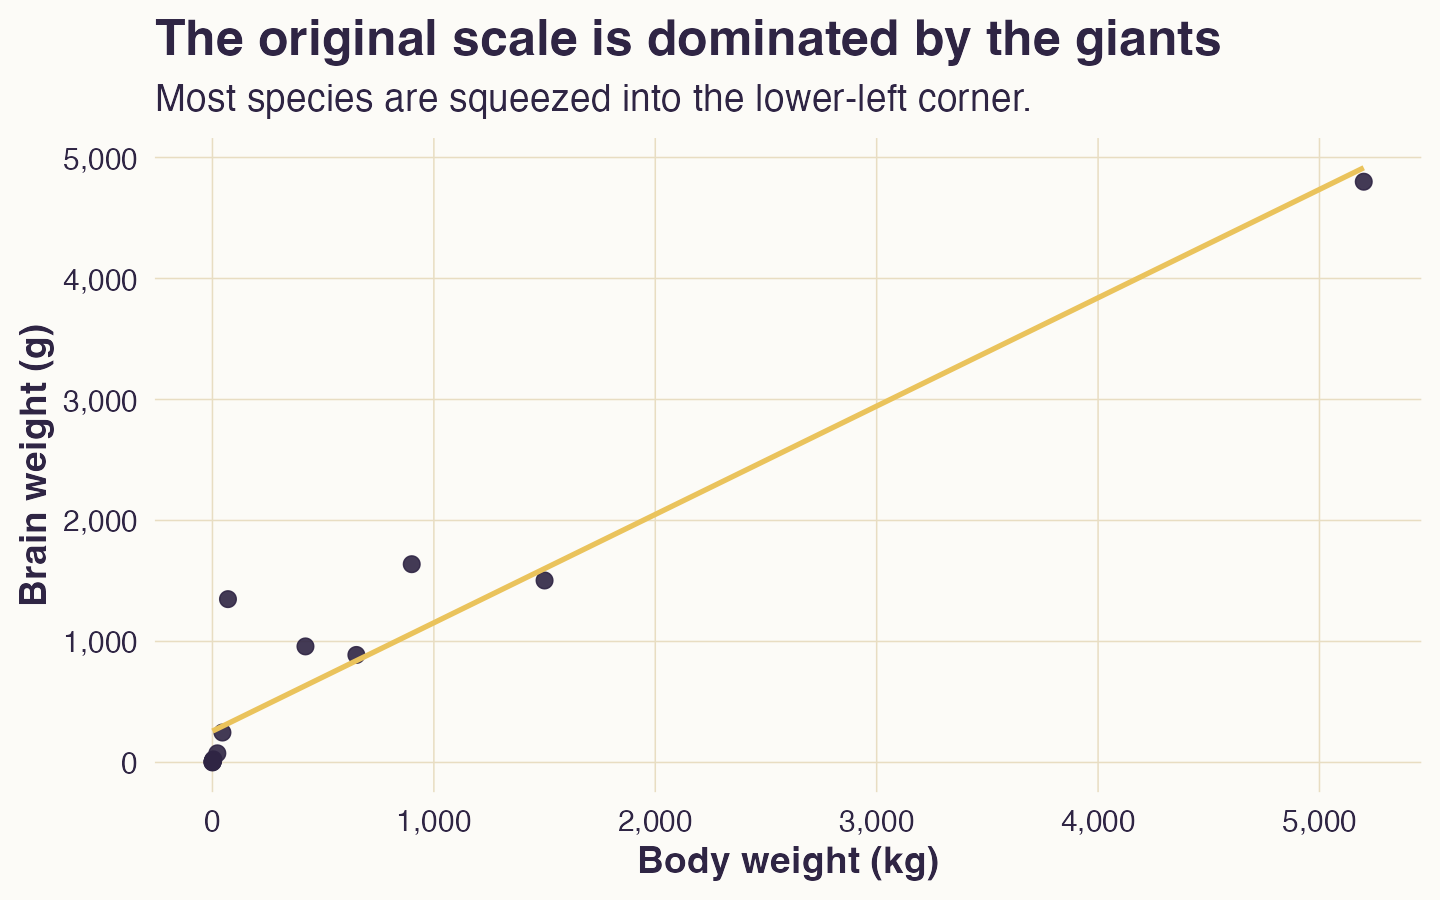
\includegraphics[width=0.86\textwidth,height=\textheight]{assets/mammals-original.png}

}

\caption{Scatterplot of mammal brain weight versus body weight on the
original scale. A few large animals dominate the axes, hiding most of
the data near the origin.}

\end{figure}%
\end{frame}

\begin{frame}{A power law}
\phantomsection\label{a-power-law}
Many scaling relationships use:

\[
y = Kx^\beta.
\]

\begin{itemize}
\tightlist
\item
  \(x\): body weight.
\item
  \(y\): brain weight.
\item
  \(K\): proportionality constant.
\item
  \(\beta\): scaling exponent.
\end{itemize}

If \(\beta = 1\), brain weight scales proportionally with body weight.

If \(\beta < 1\), brain weight grows more slowly than body weight.
\end{frame}

\begin{frame}{The log-log trick}
\phantomsection\label{the-log-log-trick}
Take logs:

\[
\log(y) = \log(K) + \beta\log(x).
\]

For mammals:

\[
\log(\text{brain}) =
\alpha + \beta\log(\text{body}) + e.
\]

This is a straight-line model for two logged variables.

The slope is an elasticity:
\end{frame}

\begin{frame}{Elasticity}
\phantomsection\label{elasticity-1}
An elasticity answers:

\begin{quote}
If \(x\) changes by 1\%, how many percent does \(y\) change?
\end{quote}

In a log-log model, the elasticity is \(\beta\).

\[
\log(y) = \alpha + \beta\log(x),
\]

The units disappear; percent talks to percent.
\end{frame}

\begin{frame}{Elasticity}
\phantomsection\label{elasticity-2}
To see why, take derivatives of both sides:

\[
\frac{d}{dx}\log(y)
=
\frac{d}{dx}\left[\alpha + \beta \log(x)\right].
\]

Using the chain rule,

\[
\frac{1}{y}\frac{dy}{dx}
=
\beta \frac{1}{x}.
\]

Rearrange: \[
\beta
=
\frac{dy / y}{dx / x}
=
\frac{\%\text{ change in } y}{\%\text{ change in } x}
\]
\end{frame}

\begin{frame}{The log-log model for mammals}
\phantomsection\label{the-log-log-model-for-mammals}
\begin{figure}[H]

{\centering 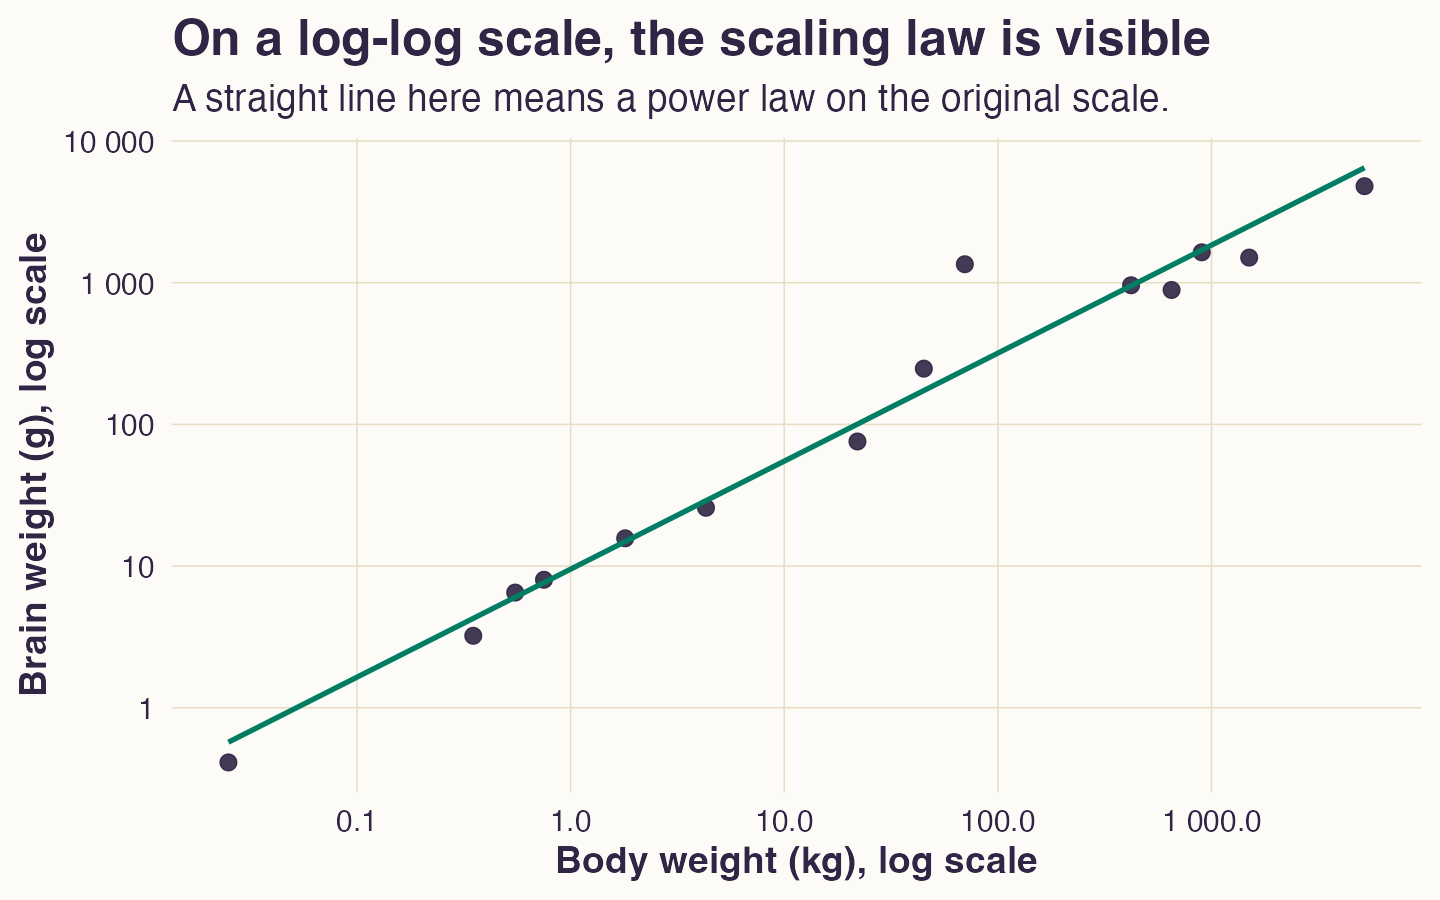
\includegraphics[width=0.86\textwidth,height=\textheight]{assets/mammals-loglog.png}

}

\caption{Scatterplot of log brain weight versus log body weight, with a
fitted line. The species form an approximately straight increasing
band.}

\end{figure}%
\end{frame}

\begin{frame}{Interpreting the mammal slope}
\phantomsection\label{interpreting-the-mammal-slope}
Suppose the fitted equation is:

\[
\widehat{\log(\text{brain})}
= 2.25 + 0.76\log(\text{body}).
\]

The elasticity is \(0.76\).

In words:

\begin{quote}
A 1\% increase in body weight corresponds to about a 0.76\% increase in
brain weight, on average.
\end{quote}

Not grams.

Percent to percent.
\end{frame}

\begin{frame}{A bigger move}
\phantomsection\label{a-bigger-move}
If body weight doubles, predicted brain weight is multiplied by:

\[
2^{0.76} \approx 1.69.
\]

So doubling body weight predicts about 69\% more brain weight.

Because \(0.76 < 1\), brain weight grows less than proportionally with
body weight.
\end{frame}

\begin{frame}{Elasticities in economics}
\phantomsection\label{elasticities-in-economics}
Examples:

\begin{itemize}
\tightlist
\item
  Price elasticity of demand: if price rises 1\%, how much does quantity
  demanded fall?
\item
  Income elasticity: if income rises 1\%, how much does spending rise?
\item
  Cross-price elasticity: if a competitor's price rises 1\%, what
  happens to your sales?
\item
  Wage elasticity of labor supply: if wages rise 1\%, how much do hours
  worked change?
\item
  Advertising elasticity: if ad spend rises 1\%, how much do sales rise?
\end{itemize}

Same grammar, different economic question.
\end{frame}

\begin{frame}{The online seller}
\phantomsection\label{the-online-seller}
An online seller runs a pricing experiment.

Visitors are randomized to see one price for the same product:

\[
\$8, \$9, \$10, \ldots, \$32.
\]

For each price, the seller records units sold.

The business question is:

\begin{quote}
If we raise price by 1\%, how much demand do we lose?
\end{quote}

That is a price-elasticity question.
\end{frame}

\begin{frame}{Demand on the original scale}
\phantomsection\label{demand-on-the-original-scale}
\begin{figure}[H]

{\centering 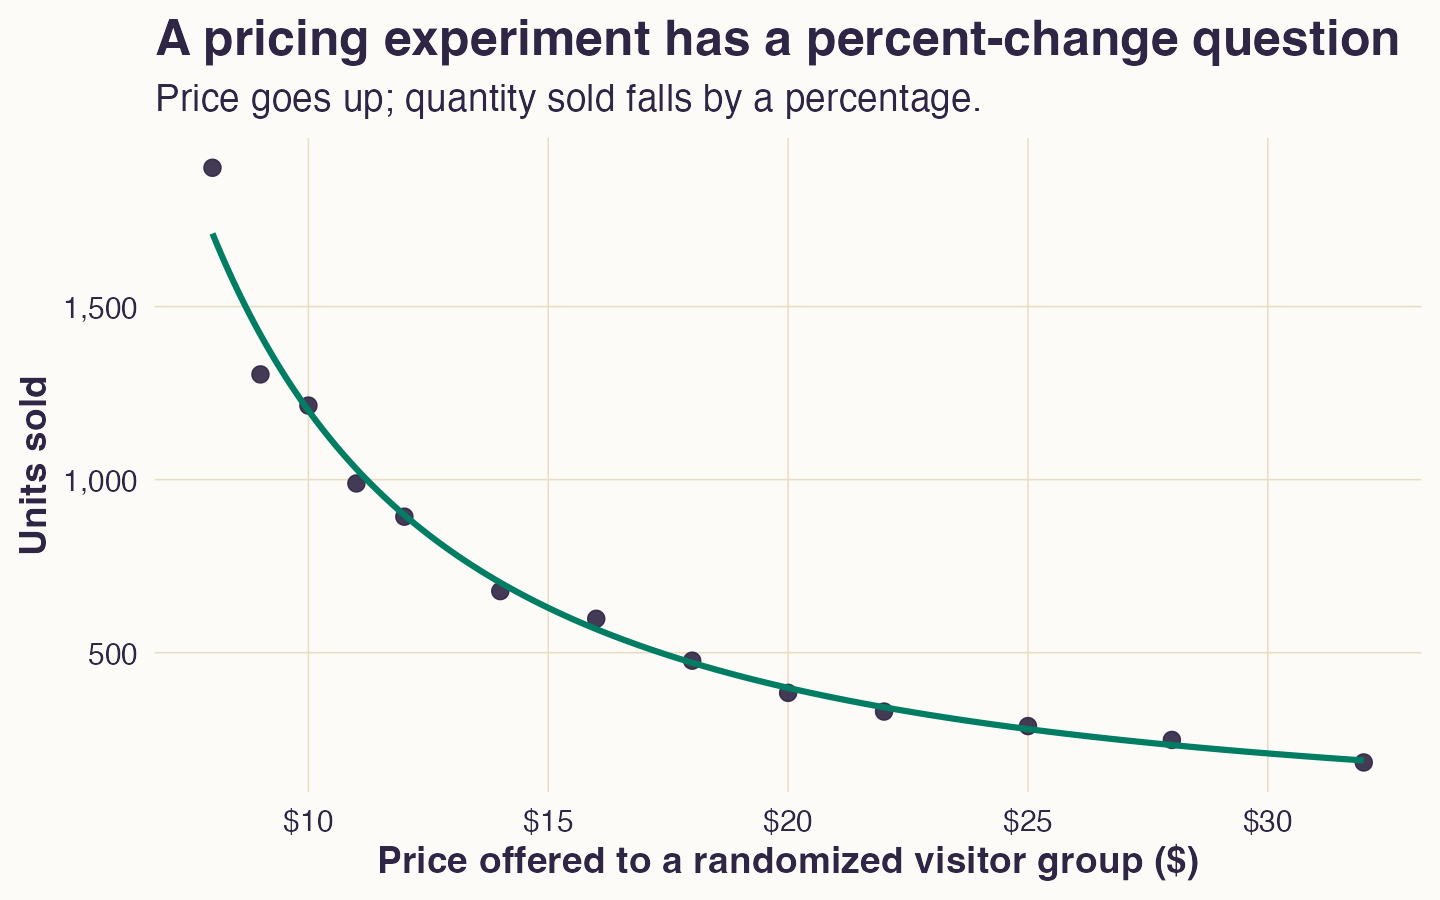
\includegraphics[width=0.86\textwidth,height=\textheight]{assets/pricing-demand-original.png}

}

\caption{Scatterplot of units sold versus randomized price, with a
downward-sloping fitted demand curve.}

\end{figure}%
\end{frame}

\begin{frame}{Demand on the log-log scale}
\phantomsection\label{demand-on-the-log-log-scale}
\begin{figure}[H]

{\centering 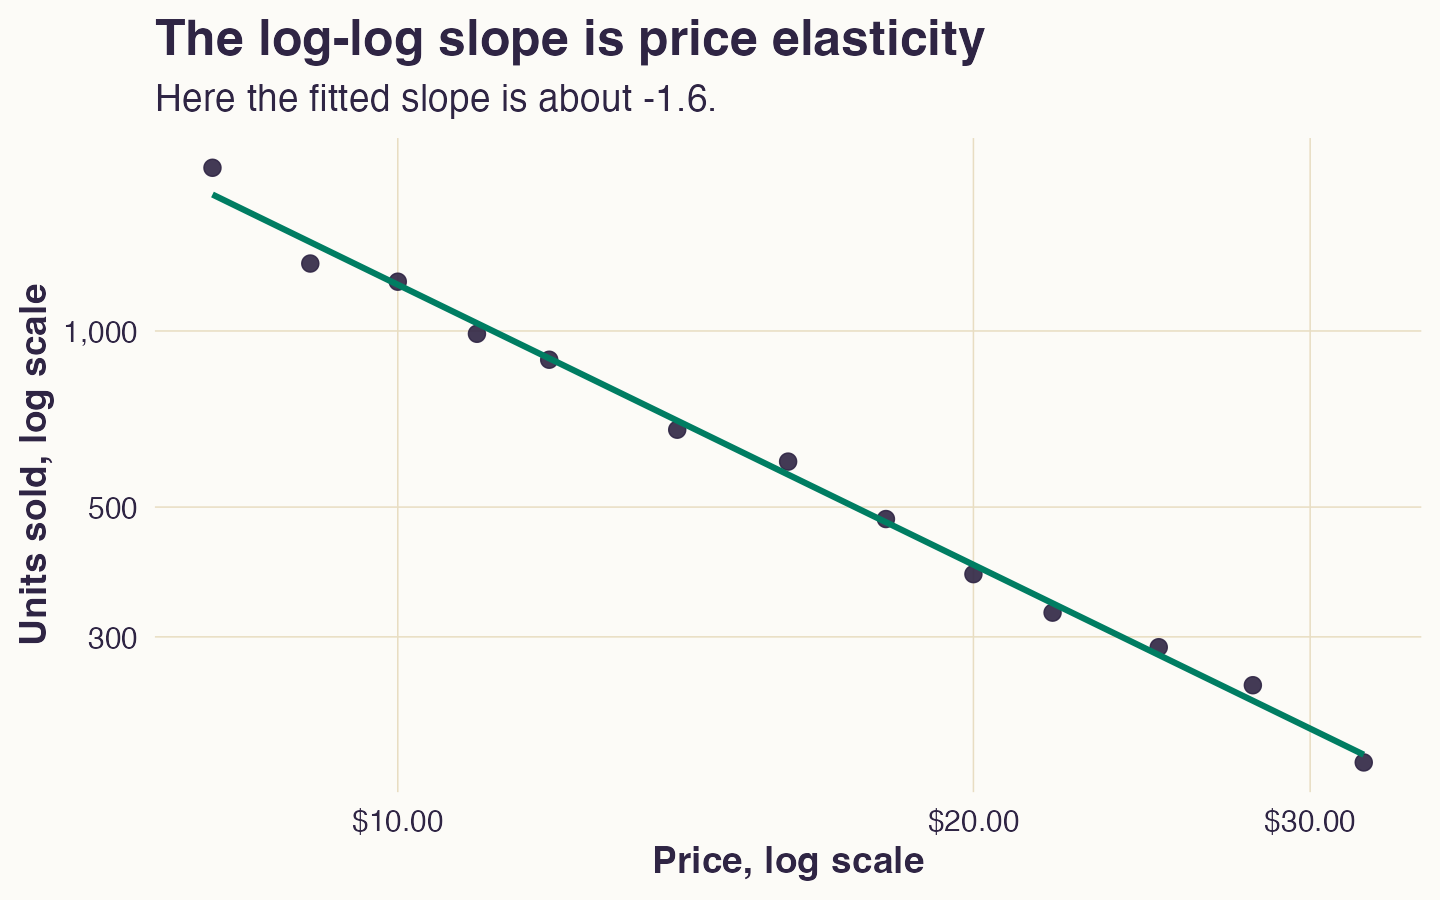
\includegraphics[width=0.86\textwidth,height=\textheight]{assets/pricing-demand-loglog.png}

}

\caption{Log-log scatterplot of units sold versus randomized price, with
a fitted line.}

\end{figure}%
\end{frame}

\begin{frame}{Reading the price elasticity}
\phantomsection\label{reading-the-price-elasticity}
Suppose the fitted equation is:

\[
\widehat{\log(\text{quantity})}
= 10.75 - 1.59\log(\text{price}).
\]

The slope is \(-1.59\).

In words:

\begin{quote}
A 1\% increase in price predicts a 1.6\% decrease in quantity sold.
\end{quote}

That is elastic demand: quantity moves more than price, in percent
terms.
\end{frame}

\begin{frame}{Why the sign matters}
\phantomsection\label{why-the-sign-matters}
Price elasticity is usually negative: higher price, lower quantity.

If the slope were \(-0.3\):

\begin{itemize}
\tightlist
\item
  a 1\% price increase predicts a 0.3\% quantity decrease,
\item
  demand is inelastic,
\item
  typically revenue tends to rise when price rises.
\end{itemize}

If the slope were \(-1.6\):

\begin{itemize}
\tightlist
\item
  a 1\% price increase predicts a 1.6\% quantity decrease,
\item
  demand is elastic,
\item
  typically revenue tends to fall when price rises.
\end{itemize}
\end{frame}

\begin{frame}{Why revenue changes}
\phantomsection\label{why-revenue-changes}
Revenue is:

\[
\text{revenue} = \text{price} \times \text{quantity}.
\]

If price rises 1\% and quantity falls 1.6\%, then revenue changes by
roughly:

\[
1\% - 1.6\% = -0.6\%.
\]

Not exact calculus, but still a good first read.
\end{frame}

\begin{frame}{Three common log models}
\phantomsection\label{three-common-log-models}
\begin{longtable}[]{@{}
  >{\raggedright\arraybackslash}p{(\columnwidth - 4\tabcolsep) * \real{0.3333}}
  >{\raggedright\arraybackslash}p{(\columnwidth - 4\tabcolsep) * \real{0.3333}}
  >{\raggedright\arraybackslash}p{(\columnwidth - 4\tabcolsep) * \real{0.3333}}@{}}
\toprule\noalign{}
\begin{minipage}[b]{\linewidth}\raggedright
Model
\end{minipage} & \begin{minipage}[b]{\linewidth}\raggedright
Fit this
\end{minipage} & \begin{minipage}[b]{\linewidth}\raggedright
Slope means
\end{minipage} \\
\midrule\noalign{}
\endhead
level-level & \(y\) on \(x\) & additive change in \(y\) per unit of
\(x\) \\
log-level & \(\log(y)\) on \(x\) & percent change in \(y\) per unit of
\(x\) \\
log-log & \(\log(y)\) on \(\log(x)\) & percent change in \(y\) per
percent change in \(x\) \\
\bottomrule\noalign{}
\end{longtable}

The model form tells you what comparison you are making.
\end{frame}

\begin{frame}{A decision rule}
\phantomsection\label{a-decision-rule}
Use logs when the question is naturally about multiplication, ratios, or
percentages.

\begin{itemize}
\tightlist
\item
  growth happens by compounding,
\item
  changes are reported as rates,
\item
  the spread grows with the level,
\item
  the original-scale plot is dominated by large values,
\item
  on a log-scale plot, the data look like they follow a linear
  relationship.
\end{itemize}

This is a modeling choice, driven by a combination of data exploration
and prior knowledge.
\end{frame}

\begin{frame}{What can go wrong?}
\phantomsection\label{what-can-go-wrong}
The common mistakes:

\begin{itemize}
\tightlist
\item
  interpreting a log-scale slope as a unit-change slope,
\item
  fitting on logs and never translating back,
\item
  using logs to hide outliers,
\item
  forgetting that errors are now ratio errors,
\item
  adding 1 to handle zeros without thinking.
\end{itemize}

The transformation is useful, but the interpretation has to follow it.
\end{frame}

\begin{frame}{The practical lesson}
\phantomsection\label{the-practical-lesson}
Logs are useful because they turn some nonlinear stories into
straight-line stories:

\[
\text{compounding} \rightarrow \text{log-response line}
\]

\[
\text{power law} \rightarrow \text{log-log line}
\]

But logging a variable changes the question.

\begin{itemize}
\tightlist
\item
  Level models speak in units.
\item
  Log models speak in percentages and ratios.
\end{itemize}
\end{frame}




\end{document}
